%===================================== CHAPTER 3 Project management =================================

\chapter{Project management}

The following chapter describes how progress of the project was planned, managing resources, controlling potential risks and assuring quality of the project and product. The project management includes a delegation of work tasks and responsibilities, risk management, a work breakdown, time management and quality assurance.

\section{Risk management}
\label{sec:risk_management}

Risk management includes planning and handling all the various potential risks to the project.\newline

The risk analysis contains a list of possible occurrences that could be harmful to the project. Provided for each risk is a short description, an estimated likelihood that the risk will happen, an estimated impact to the project if it happens, the importance of the risk, a preventive action to try to avoid the problem and a remedial action if the problem were to occur. Likelihood and impact estimates were rated on a scale from 1 to 9, with 9 being the highest, and the importance was calculated by multiplying likelihood with impact. The risk list is sorted by the importance value, thus the risk to be most aware of at each stage of the development process was at the top of the list. Risks were updated regularly and changes were made when new issues were discovered.\newline

\textbf{Table \ref{Tab:riskexample}} describes three of the most important risks in the risk analysis. The complete risk analysis is located in \textbf{Appendix \ref{app:risklist}}.

L: Likelihood (1-9)\\
I1: Impact (1-9)\\
I2: Importance (Likelihood * Impact)\\

\begin{table}[!h]
\begin{center}
	\caption{Risk list example} 
	\label{Tab:riskexample}
	\begin{tabular}{ | p{3.5cm} | p{2cm} | p{1.5cm} | p{2cm} | p{3.5cm} | p{3.5cm}|}

		\hline
		\textbf{Description} & \textbf{L} & \textbf{I1} & \textbf{I2} & \textbf{Preventive action} & \textbf{Remedial action} \\ \hline
		
		Underestimate the time planned to use for assignments & 8 & 8 & 64 & Estimate a little higher. continuous meetings. Continuous status update on tasks & Extra work hours and help each other. Have a clear prioritization of tasks so that some less important tasks can be delayed if needed. \\ \hline
		
		The group does not deliver updated information on the report and cannot maximize the quality of the feedback obtained from the supervisor & 6 & 7 & 42 & Always make sure the report meet the demands upon delivery & Ask concrete questions to the supervisor or other competent acquaintances of the group members \\ \hline
		
		An issue in the code that is not understood or can not be fixed. & 5 & 8 & 40 & Comment on the code, and talk with each other about the work done on the code & Get help from the supervisor or other people involved. \\ \hline
	\end{tabular}
\end{center}
\end{table}

\section{Meetings}
\label{sec:meetings}

The group had many meetings with parties that were involved with the project and/or the application. The three main types of meetings documented were group meetings, customer meetings, and supervisor meetings.\newline 

It became a logical decision to make use of scrum to have 1-week sprints, which would include daily scrum meetings with the group. Since the team was a group of seven, it was impossible to always work together. Because of this, the regular scrum meetings were beneficial to share and discuss progress. During each meeting, a summary was written to document what the group members had done since last, what issues had occurred, and any other important notes. An example of a group meeting report can be found in \textbf{Appendix \ref{app:meetingreport}}.\newline

The customer requested weekly meetings, and to make the most out of these meetings, the team planned an agenda ahead of each meeting. This was done to improve the structure of the meeting and to give the participants time to consider the issues on the agenda, which in turn was meant to increase the benefits of the meeting and increase the likelihood of making decisions. During the meetings, a summary was written as well. An example of a customer meeting report can be found in \textbf{Appendix \ref{app:meetingreport}}.\newline

The supervisor requested bi-weekly meetings which were used to discuss the report. The supervisor read the most recent version of the report in advance of each meeting and gave feedback on what needed to be changed. Because of this, after each meeting the team kept a list of feedback from the supervisor of issues that should be handled before the next supervisor meeting. Status reports were also made and sent to the supervisor before each meeting, and an example of a status report can be found in \textbf{Appendix \ref{app:status_report}}

\section{Scrum team and roles}
\label{sec:scrum_team_and_roles}

The role delegation in the team is detailed in \textbf{Table \ref{Tab:roles}}. The delegation of roles was primarily based on personal interest and motivation. The tasks were divided up into main responsibility areas for back-end and front-end before assigning people to each one. However, this was only a guideline for main responsibilities, and the group members had to be flexible and work with tasks outside of their main areas.

\begin{table}[!h]
	\small
	\centering
		\caption{Role delegation}
		\begin{tabular}{ | p{2.5cm} | p{2.8cm} | p{12cm} |}
			\hline
			\textbf{Role} & \textbf{Responsible} & \textbf{Details} \\ \hline
			
			\textbf{Product Owner} & Jacqueline Floch (SINTEF) \newline Shanshan Jiang (SINTEF) & \\ \hline
			
			\textbf{Group supervisor} & Soudabeh Khodambashi & \\ \hline
			
			\textbf{Main back-end staff} & Hanne Marie, Eivind, Kjersti, Audun & \\ \hline
			
			Interaction between server modules & Hanne Marie & This involves making the different server components communicate and work together, such as the database, personalization module, Docker file, etc. \\ \hline
			
			Personalization & Eivind & Involves the procedure for taking a user's context information and preferences, and based on this choose which stories to present to the user. Also involves collaborative filtering to select stories for a user based on the preferences of other users. \\ \hline
			
			Test responsible & Kjersti & Involves creating a test plan for each kind of test (unit, usability, integration, etc.) and documenting the results, as well as assuring test quality and that the tests are actually conducted properly. \\ \hline
			
			Database Manager & Audun & Involves setting up and managing the database. Manage which elements to save in the database and how to present the data upon request. \\ \hline
			
			\textbf{Main front-end staff} & Ragnhild, Roar, Espen & \\ \hline
			
			iOS responsible & Ragnhild & Involves developing and giving the app a look and design that feels intuitive and follows design conventions according to iOS systems. This is both on a technical and design level. \\ \hline
			
			Android responsible & Roar & Involves developing and giving the app a look and design that feels intuitive and follows design conventions according to Android systems. This is both on a  technical and design level. \\ \hline
			
			Framework responsible & Espen & Involves developing various parts of the UI, and researching the framework to ensure that the front-end design can be made and is made according to the team's and customer's expectations. \\ \hline
			
			\textbf{Additional roles} & Roar, Kjersti, Espen & \\ \hline
			
			Scrum Master & Roar & Project leader, responsible for arranging meetings, delegating work tasks, and overseeing the general progress of the project. Facilitate the communication and cooperation between the group members. \\ \hline
			
			Customer relations & Kjersti & This includes all communication with the customer, as well as other authorities that are a part of the project. \\ \hline
			
			Report management & Espen & This involves overseeing the report work and ensuring that all components of the report are in place. Deliver the report within deadlines and make changes as needed and in accordance with advice from supervisor. \\ \hline
		\end{tabular}
	\label{Tab:roles}
\end{table}

\section{Work breakdown structure}

A work breakdown structure is a decomposition of the project, and its goal is to break down each part of the development process into manageable parts to ease the planning and execution of the development. Each element in the diagram can be a product, data, service or a combination of the three. One of the benefits of detailing a project this way appears when doing cost estimation and scheduling the team around the project (i.e. should ease the project planning and help allocate the team's resources).\newline

The work breakdown structure shows a hierarchical decomposition of the project phases and its components. Each main phase is at a top-level and will outline the generic parts of the software development processes. The way the WBS (Work Breakdown Structure) is developed is by starting with the end objective and subdividing each main part into manageable components in terms of size, complexity and duration. Each sub objective is to follow the 80 hour rule. This means that a subtask is not to exceed 80 hours in magnitude. The WBS for this project is shown below in \textbf{Figure \ref{Fig:wbs}}. %% For a brief description on what is intended for each package see \textbf{Appendix \ref{app:wbs_description}}.

\begin{figure}[h!]
	\begin{center}
		\advance\leftskip-3cm
		\advance\rightskip-3cm
		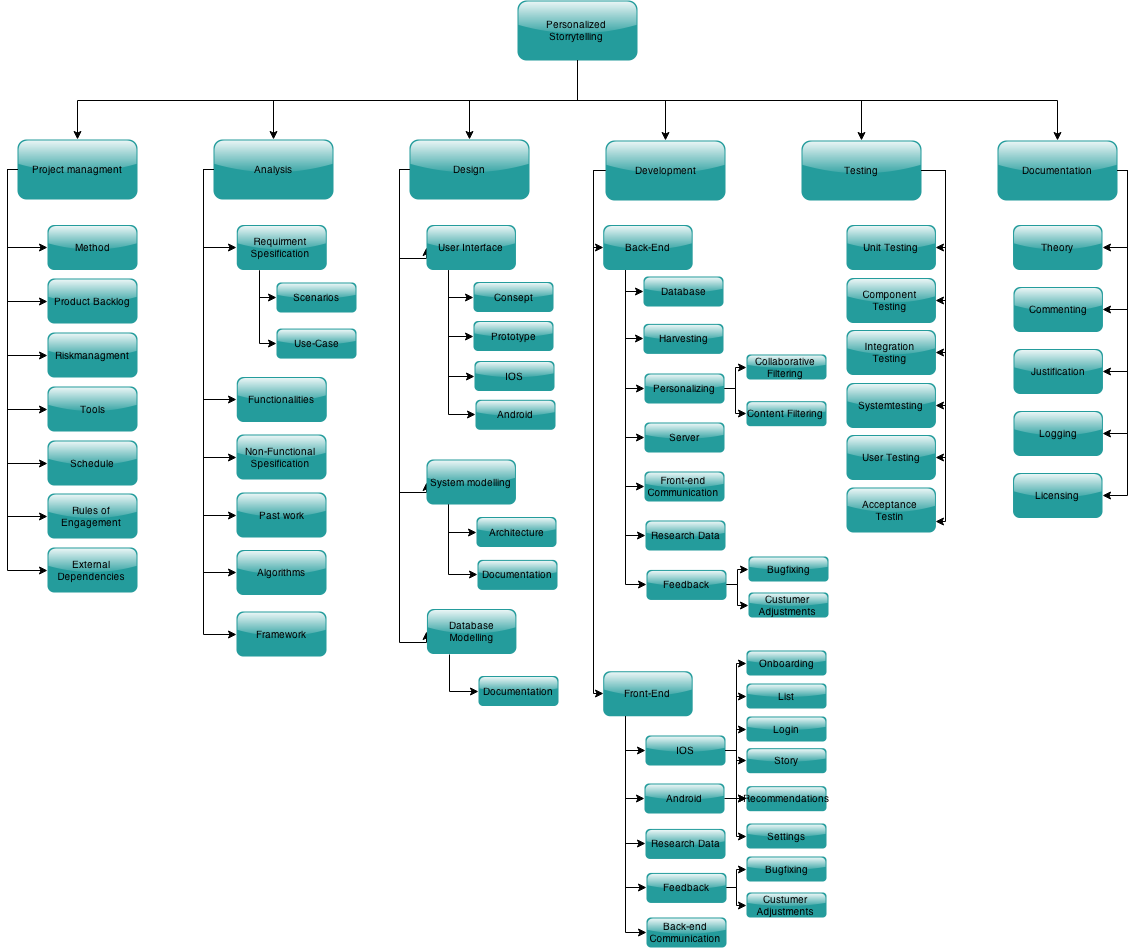
\includegraphics[keepaspectratio=true,scale=0.43]{fig/wbs}
		\caption{Work breakdown structure}
		\label{Fig:wbs}
	\end{center}
\end{figure}

\section{Project milestone plan}
\label{sec:milestone_plan}

Milestones are used as tools in project management to give the team some clear and specific goals to work towards as the project timeline moves ahead. There are several milestones throughout the project, some are large milestones, like the alpha and beta versions of the software. There are also milestones related to the project report, like the midterm submitting and final delivery. Milestones can add some value to the project scheduling when used in the right manner and when setting realistic goals. Components that are important for the milestone plan are; key dates, key deadlines and external deliveries. The team used a combined Gantt chart with milestones noted for better visualization, and to better allocate resources for meeting the milestone goals. The Gantt chart is presented in Figure \textbf{\ref{Fig:gantt}}.\newline


The planned deliveries to the customer are the following dates. 
\begin{itemize}
\item \textbf{20.02.15 - First prototype} \newline
A prototype should be finished by this date. Paper or mockup would suffice  
\item \textbf{27.02.15 - Second prototype}  \newline
The next iteration of the prototype should be presented in proto.io \cite{protoIO}
\item \textbf{17.03.15 - Alpha} \newline
First working software should be ready for a customer test
\item \textbf{10.04.15 - Beta}  \newline
A feature ready version of the application should be ready for the customer 
\item \textbf{01.05.15 - Final product} \newline
A polished and well tested application and ready to deploy back-end should be ready for delivery 
\end{itemize}

\todo{forklar hvordan man kom fram til dette?, legg hele gantt til i appendix?}

\begin{figure}[h!]
	\begin{center}
		\advance\leftskip-3cm
		\advance\rightskip-3cm
		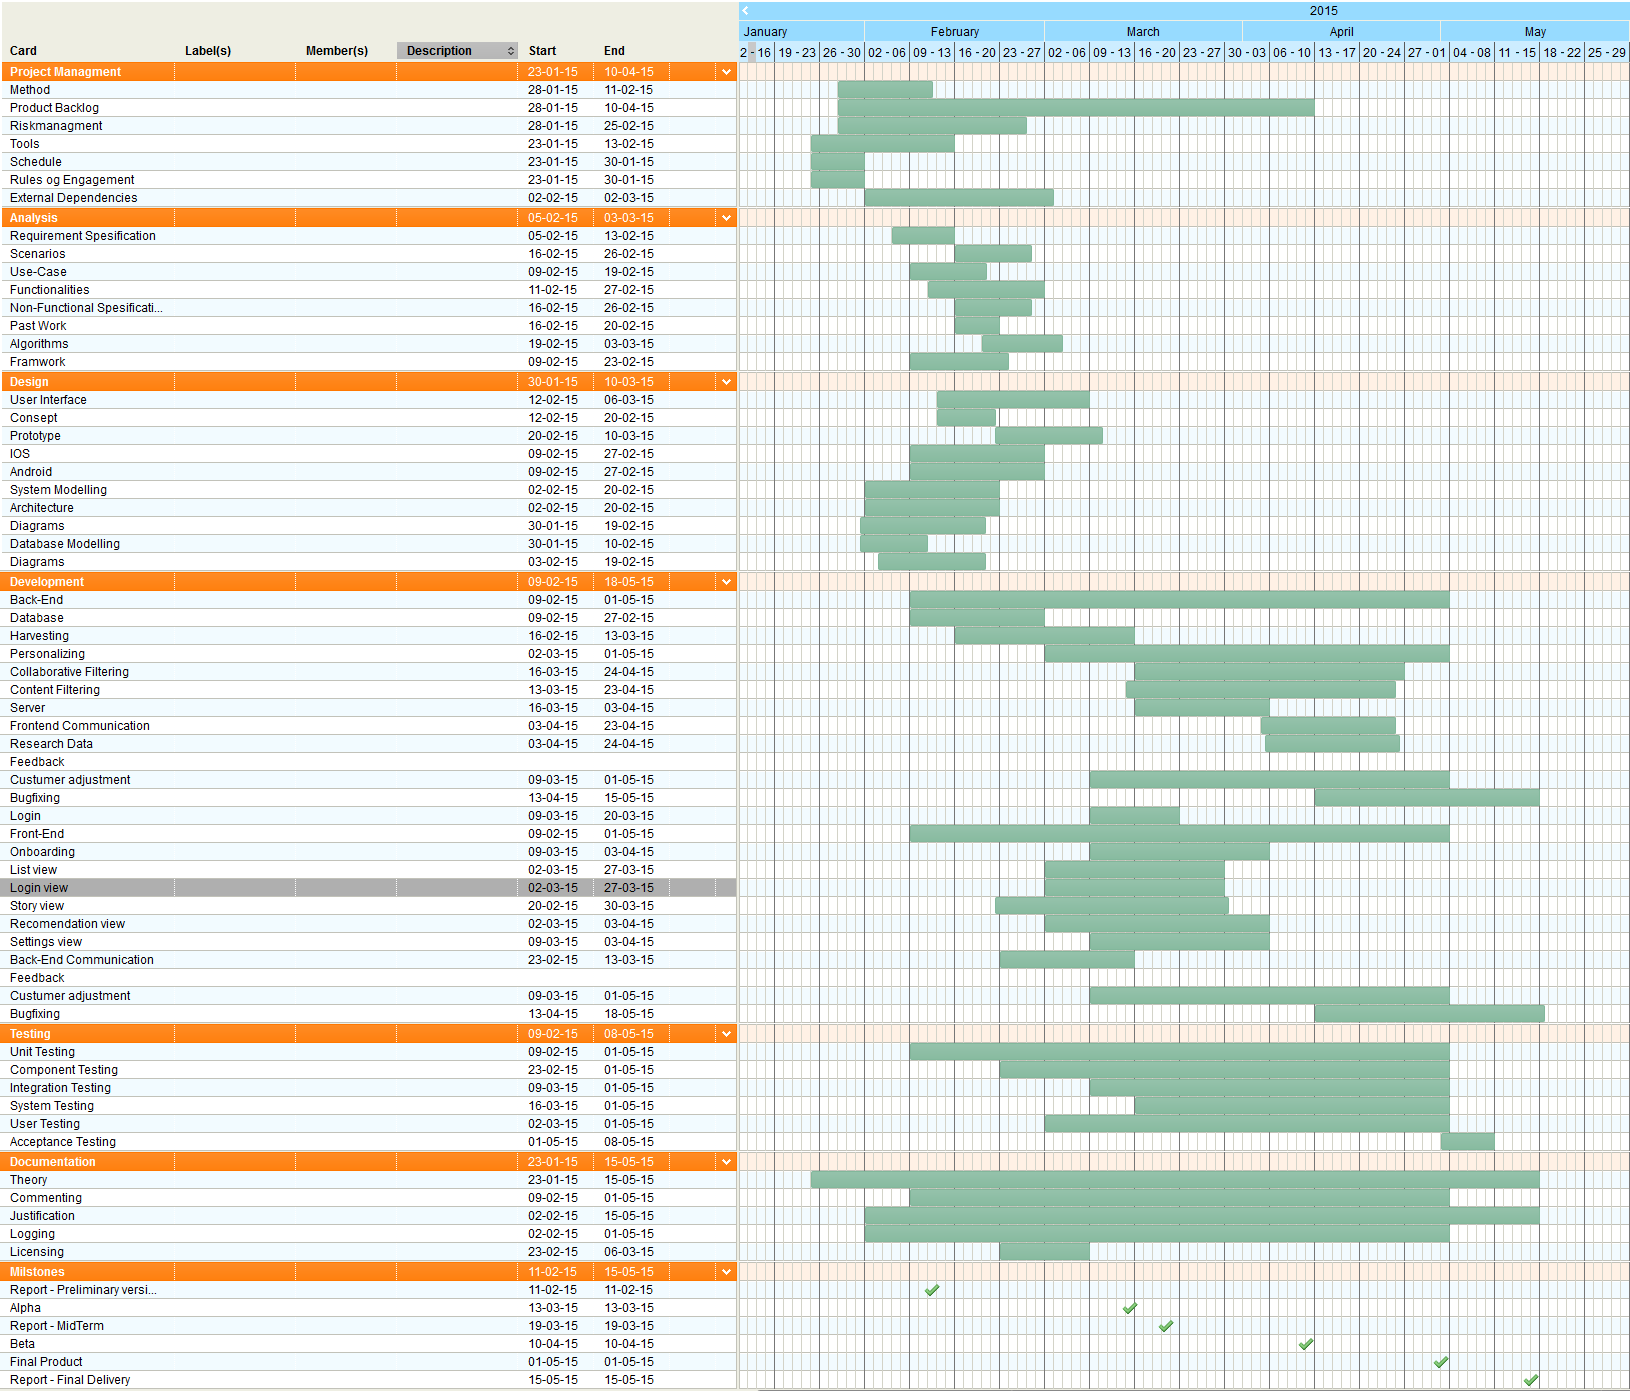
\includegraphics[keepaspectratio=true,scale=0.5]{fig/gantt}
		\caption{Gantt chart}
		\label{Fig:gantt}
	\end{center}
\end{figure}

\section{Burn down}

\todo{Skrive om activity plan}

A burn down chart is a visual representation of the outstanding work(Appendix \ref{app:activity_plan}) relative to the projects remaining time. Its visual representation is outlined in a graph where the x-axis represents the timeline where each point on the graph is one sprint, and the y-axis represents the estimated hours needed to finish the project. This is useful to have a better understanding of the rate that the project is moving and it indicates whether or not one will meet the project's estimates.\todo{Skal vi sitere her? http://idiacomputing.com/pub/BetterSoftware-BurnCharts.pdf, http://joel.inpointform.net/software-development/burn-down-charts-tutorial-simple-agile-project-tracking/  }\newline

Our estimates were done on the basis that each team member would have a workload of about 20 hours each week. \todo{Dette ble sagt i forelesning. Men på nettet står det 24 timer?, har sendt mail til Monica}


The burn down estimate done at the start of the project can be found in \textbf{Figure \ref{Fig:burndownstart}} below. The final burn down of the project can be seen in \textbf {Figure \ref{Fig:burnDownAfter}}.



\begin{figure}[h!]
	\centering
	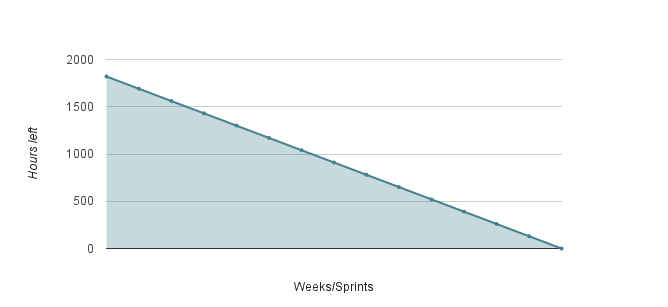
\includegraphics[width=\textwidth]{fig/burndownstart}
	\caption{Estimated burn down chart}
	\label{Fig:burndownstart}
\end{figure}


\section{Quality assurance}

According to Sommerville, quality assurance is “the definition of processes and standards that should lead to high-quality products and the introduction of quality processes into the manufacturing process” \cite[p.652]{Sommerville}. In large systems designed to be used in a long term perspective, quality documentation is important. However, in this project a smaller system was developed and Sommerville notes that a more informal approach can then be applied, focusing on “establishing a quality culture” \cite[p.654]{Sommerville} within the development team.\newline

Therefore, this section will describe four features considered important by the group to establish such a quality culture, and thus improving the quality of the product, namely group interaction, version controlling, code quality and interaction with the customer. Risk management and testing are also considered important aspects of quality assurance, and these are discussed in separate parts (see \textbf{Section \ref{sec:risk_management}} for risk management and \textbf{Chapter \ref{chap:testing}} for testing). 

\subsection{Group interaction}

As was noted in \textbf{Section \ref{sec:scrum}}, an important part of the scrum methodology is the close collaboration between the team members. Scrum provides some events to enhance this collaboration, for instance the daily scrum meetings, and some artifacts, such as the sprint backlog. These features of scrum were used by the group and helped create a framework for the process development. However, scrum does not define how the group should interact, and the group interaction consisted of more than the methods provided by scrum, for instance when doing sessions of collaborative work.\newline

In order to ensure that the scrum events and the interactions external to these events would create the desired quality culture, the team discussed and agreed upon some basic rules of engagement for the project (see \textbf{Appendix \ref{app:rules_of_engagement}}). These rules specified how the team should create a quality process in order to create a quality product, for instance by setting ground rules for communication between the group members. The tools described in \textbf{Section \ref{sec:communication tools}} were used to facilitate the implementation of the rules. In addition, meeting minutes from every meeting were made so that every group member would be aware of the status of the project even if they were not present at the meeting.\newline

The division of the group described in \textbf{Section \ref{sec:scrum_team_and_roles}} meant that a member of the front-end part would have more detailed information about what other front-end developers were doing than what individual members of the back-end part were doing, and vice versa. However, when important decisions were to be made in one part of the project or important problems had to be solved, both parts would be involved in the discussion, even if the decision did not affect their part of the project directly. An example of such a decision was the choice of colors to use in the user interface.

\subsection{Git and version controlling}

The code for this project is hosted by GitHub, a tool described in \textbf{Section \ref{sec:additional_tools}}. GitHub uses the version control system Git, which makes development easier by allowing multiple local branches and thereby giving users the opportunity to try out code before committing it to the master branch. The master branch is the main branch and should only include stable code. The group chose to create two repositories, one for the back-end part of the project and one for the front-end part, since the group was divided in this way as well. Doing it this way made keeping track of branches and issues on GitHub clearer since these often would be at a level of detail only relevant to the developers in that part of the project. 

\subsection{Code quality}

In order to ease the cooperation on the code for the project, the group followed some general guidelines. These guidelines were:
\begin{itemize}
	\item Use descriptive names on variables, classes, folders and other elements
	\item Comment code
	\item Divide the code into logical units (Section \ref{sec:frontend_structure})
	\item Make sure the code units are not too large
\end{itemize}

\subsection{Customer interaction}

In \textbf{Section \ref{sec:scrum}} it was noted that the project was flexible and likely to have changes in the requirements. This meant that good customer interaction was critical, so that the group and the customer would be in agreement of what was expected of the end product. The customer meetings are described in \textbf{Section \ref{sec:meetings}} and apart from these meetings, communication with the customer was also done by mail and by a shared Dropbox folder. In addition, the customer were by their request watchers of the code on GitHub. \newline

Making decisions and coming to an agreement with the customer on key issues was considered important to push the project forward. The meeting minutes written after each meeting allowed the customer to know if all the participants had a similar understanding of the issues discussed and the decisions made. Communication by mail was mainly used for rescheduling of meetings and by the customer to give additional information to the group. 

\cleardoublepage